\section{Experimental setup}
\label{sec::experiments}

The experimental phase aims at testing the proposed framework in a highly controlled environment, where we focus on learning the mapping between image descriptors and motor-sensor data to predict the grasp associated to each object. In the following we present the experimental setup and the regression results.

\subsection{Data acquisition setup}
\label{sec::acquisition}

Data were collected using two Watec \emph{WAT-202D} colour cameras for the images and a  Immersion \emph{CyberGlove} with $22$-sensors for the hand posture. An Ascension \emph{Flock-Of-Birds} magnetic tracker mounted on the subject's wrist, and an additional standard force sensing resistor glued to the subject's thumb were used to determine the hand position and speed, and the instant of contact with the object.\\
\begin{figure}[h!]
	\centering
	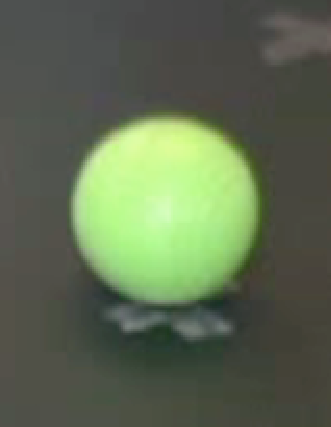
\includegraphics[height=1.75cm]{images_pdf/images/palla}
	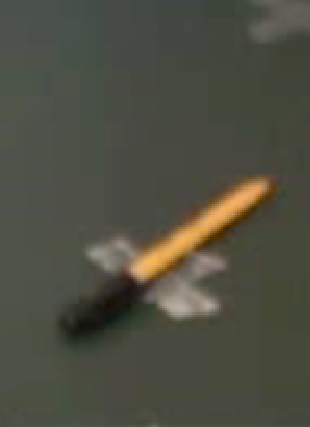
\includegraphics[height=1.75cm]{images_pdf/images/penna}
	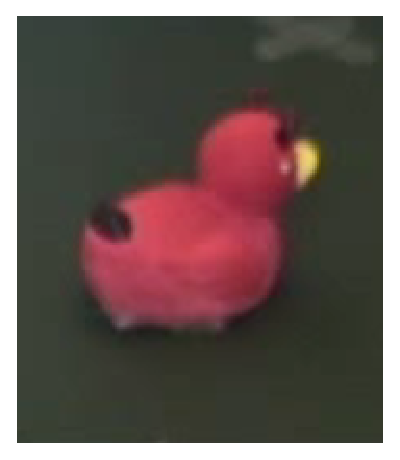
\includegraphics[height=1.75cm]{images_pdf/images/papera}
	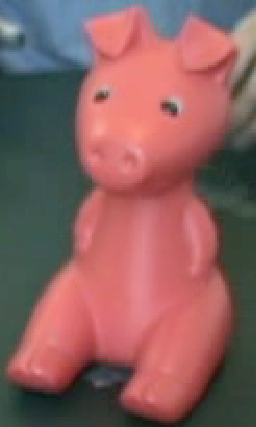
\includegraphics[height=1.75cm]{images_pdf/images/porcellino}
	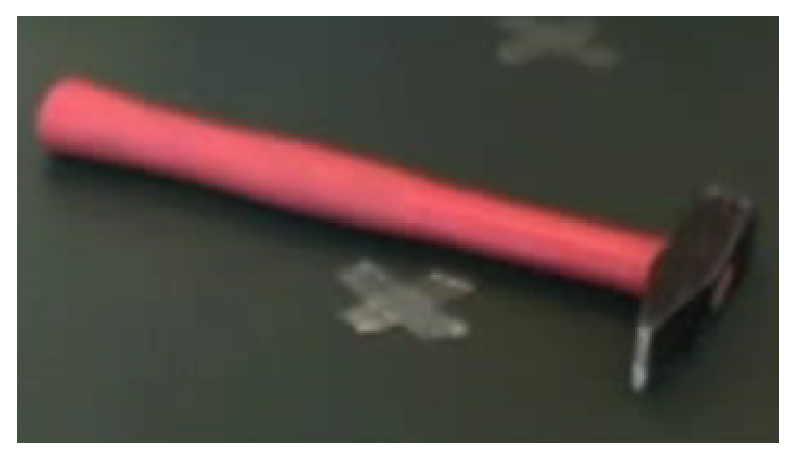
\includegraphics[height=1.75cm]{images_pdf/images/martello}
	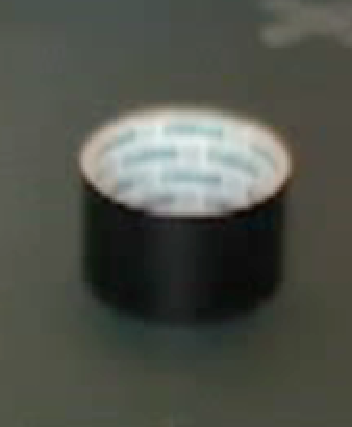
\includegraphics[height=1.75cm]{images_pdf/images/scotch}
	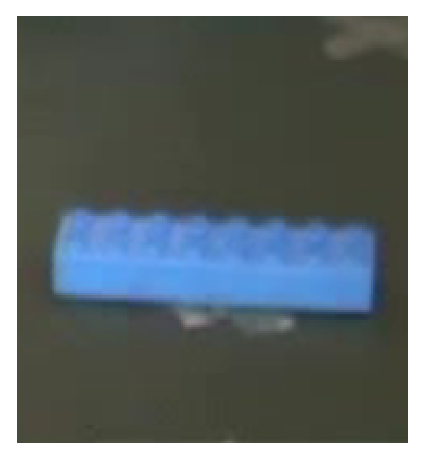
\includegraphics[height=1.75cm]{images_pdf/images/lego}\\
	\vskip 0.1cm
	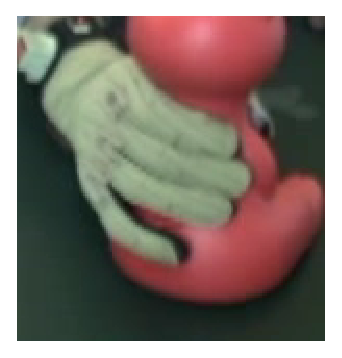
\includegraphics[width=0.19\textwidth]{images_pdf/images/cylinder}
	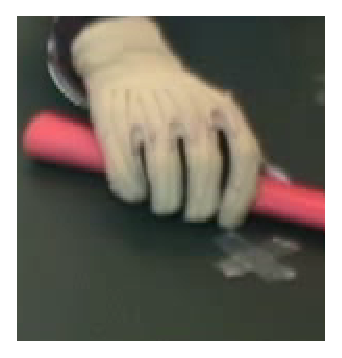
\includegraphics[width=0.19\textwidth]{images_pdf/images/flat}
	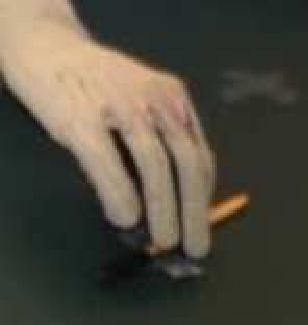
\includegraphics[width=0.19\textwidth]{images_pdf/images/pinch}
	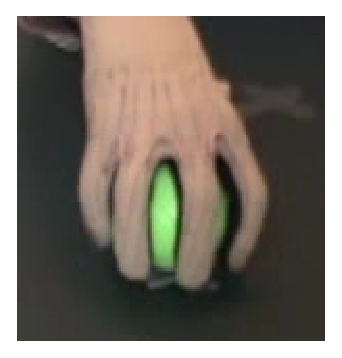
\includegraphics[width=0.19\textwidth]{images_pdf/images/spherical}
	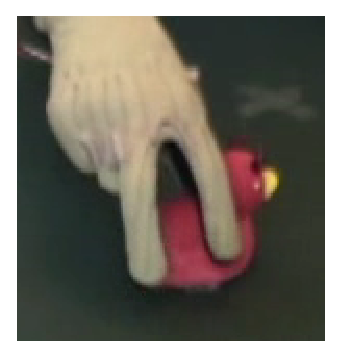
\includegraphics[width=0.19\textwidth]{images_pdf/images/tripodal}
	\caption{Top row: the objects used in our experiments. Bottom, the grasp types we consider: \emph{(left to right)} cylindric power grasp, flat grasp, pinch grip, spherical and
	tripodal grip.}
	\label{fig::grasps}
\end{figure}

The cameras return two video sequences, one placed laterally with focus on the object (the \emph{spectator}) and one placed in front of the subject (observing the \emph{actor}). We process only the {\em spectator} video sequence, because it supplies all the information required for preliminary testing. The video sequence is acquired at $25$Hz by each camera, while the glove is sampled at $100$Hz. Since the three devices are independent of one another a system of common time-stamps was used in order to synchronise the data.\\
The CyberGlove returns $22$ $8$-bit numbers linearly related to the angles of the subject's hand joints. The resolution of the sensors is on average about $0.5$ degrees. The sensors describe the position of the three phalanxes of each finger
(for the thumb, rotation and two phalanxes), the four finger-to-finger
abductions, the palm arch, the wrist pitch and the wrist yaw.\\
For these preliminary experiments we considered $7$ objects and $5$ grasping types identified by different hand postures (see Fig. \ref{fig::grasps}); $2$ subjects have joined the experiment: for each object, the actor was asked to perform the required grasping action $20$ times. 

\subsection{Proof of concept experiments}
Among the motor data, it is reasonable to consider only the 22 measures of hand joints as the most relevant for accurately describing the intrinsic properties of each grasping type.
When a grasp occurs the pressure on the force sensing resistor increases, causing the signal to vary hence fixing the time-stamp 
of the event. Concurrently the values on each hand joint are stored as our output data.

By synchronising motor data and video sequence we select as input data the frames showing an object without clutter, going back along the sequence from the time-stamp in which the event occurs for a fixed amount of frames (see Fig. \ref{fig::vision}, left). 
Our data are thus generated as pairs of image descriptors and sensor-motor values, respectively input and output used to feed the regression model. 

The regression methods discussed in Sec.\ref{sec::regression} are implemented in order to predict the expected sensor values of a grasp given the image of an object to be grasped. 
We compare four different image representations, based on bag-of-words descriptors where the histograms are computed for $20$ and $50$ words vocabularies on the entire image or on its four quadrants and then concatenated. We call the representations W20, W20conc, W50 and W50conc.\\
We consider two settings to evaluate the prediction performance of the proposed algorithms. In the first setting (V1-V2) we build training and test sets with the first and second volunteer's data respectively ($140$ examples each). In the second setting (MIXED) we mix the data of both volunteers and perform a 5 fold cross validation (5-CV). For both settings 5-CV on the training data only is used to select the regularizing paramenter for the RLS method and the stopping iteration for the Landweber 
\cite{bulmann02boosting,LoGerfo08Spectral} and $\nu$-method \cite{LoGerfo08Spectral}. The optimal regularization parameter is chosen among $25$ values ranging from $10^{-6}$ to $10^{-2}$, according to a geometric series. The maximum number of iterations for the iterative methods is set to $800$.
Tab.\ref{tab:results} summarizes the prediction errors evaluated according to the square loss on all $22$ components.
The prediction errors are consistent among the three learning methods, homogenous with respect to the setting and there are no significant differences among the four representations.
The values for the second setting are markedly lower because mixing the data of both volunteers reduces the variance between training and test sets in each split of the 5-CV. Therefore if we aim at building a model generalizing on several people, it is crucial to collect data from a large variety of volunteers.\\
\begin{table}[h!]
\centering

\begin{tabular}{|c|c|c|c|c|c|c|}
\hline 
\multirow{2}{*}{Setting} & \multirow{2}{*}{Representation}  & RLS  & \multicolumn{2}{c|}{Land}  & \multicolumn{2}{c|}{$\nu$-method}  \\\cline{4-7}
 & & err $ [10^3]$ &err $ [10^3]$ & iterations& err $ [10^3]$ &iterations\\\hline
\multirow{4}{*}{V1-V2} & W20conc  & $48$ & $47$& $630$ & $47$&$60$\\\cline{2-7}
&W20  	  & $37$ & $38$& $580$ &$38$&$60$\\\cline{2-7}
&W50conc & $41$ & $40$&  $340$&$40$&$30$\\\cline{2-7}
&W50 	  & $43$ & $43$&  $540$ &$43$&$40$\\\hline
\multirow{4}{*}{MIXED} 
& W20conc & $6.1 (1.1) $ & $6.4 (1.2) $& $670$ &$6.4 (1.2) $&$80$\\\cline{2-7}
& W20 & $7.9 (1.3) $ & $8.0 (1.2) $& $630$ &$8.0 (1.3) $&$70$\\\cline{2-7}
&  W50conc &   $6.1 (0.8) $ & $6.1 (0.9) $& $630$ & $6.3 (0.7) $&$70$\\\cline{2-7}
& W50 & $7.4 (2.0) $ & $7.2 (2.0) $& $620$ &$7.3 (2.0) $&$60$\\\hline
\end{tabular}
\caption{Data analysis results. 
We considered two different settings, which differ on the data splitting between training and test sets. 
Four distinct visual data representations are compared by feeding three learning methods, namely regularized least square (RLS), Landweber (Land) and $\nu$-method (see text for details). 
For each method we report the prediction accuracies expressed as mean square error and the average number of iterations for the iterative methods. 
In the MIXED setting the associated variance is reported as well. Results are consistent among the different learning techniques. }
\label{tab:results}
\end{table}
Finally, we aim at classifying the grasp type given the estimated sensor values.
We restrict at the MIXED setting, using the best regression outcome case,  W50conc/RLS.
The input data are the sensor measures and the output data are the grasp classes.
Again, a 5-CV is performed. For each split the training set is the actual set of measures from the sensors paired with the corresponding
grasp type, while the test set is the set of estimated measures.  
We train a RLS classifier \cite{rifkin03rlsc} in a One-vs-All configuration 
 obtaining a prediction accuracy of 99.6 (0.8)\%. 
 This result indicates that the regression models perform well and 
 guaranteeing the validity of the idea underlying the framework.









